% !TEX TS-program = arara
% arara: clean: {files: [ elaborat.aux, elaborat.bbl, elaborat.toc]}
% arara: xelatex
% arara: nomencl
% arara: biber
% arara: biber
% arara: xelatex
% arara: xelatex
% arara: clean: {files: [elaborat.aux, elaborat.bbl, elaborat.toc, elaborat.nls, elaborat.nlo, elaborat.ilg, elaborat.bcf, elaborat.blg, elaborat.out, elaborat.run.xml, elaborat.lof]}
%
%
%
\documentclass[german,12pt,oneside,titlepage,listof=totoc,bibliography=totoc]{scrartcl}
\usepackage[a4paper, left=4cm, right=2cm, top=4cm, bottom=2cm]{geometry}
%====================================
% Layout Pakete
%====================================
\usepackage{float}
\usepackage{fancyhdr}
\usepackage{fancybox}
\usepackage{setspace}
%====================================
% Sprachsupport Pakete
%====================================
\usepackage[ngerman]{babel}
\usepackage[T1]{fontenc}
\usepackage{polyglossia}
\setdefaultlanguage[spelling=new]{german}
\usepackage[german=quotes,autostyle]{csquotes}
%====================================
% Divers
%====================================
\usepackage{threeparttable}
\usepackage{longtable}
\usepackage{pdfpages}
\usepackage{appendix}
\usepackage{pdfsync}
\usepackage{blindtext}
%====================================
% Systemschriftarten Pakete
%====================================
% eine Times new Roman Version
%====================================
\usepackage{fontspec}                   % muss vor den Schriften ausgeführt werden
\setmainfont{Times New Roman}
\defaultfontfeatures[\rmfamily,\sffamily]{Ligatures=TeX}
\addtokomafont{sectionentry}{\mdseries} % keine Fettschriften im Inhaltsverzeichnis
\setkomafont{sectioning}{\bfseries}     % Überschriften mit Serifenschrift
\usepackage{anyfontsize}
\usepackage{ragged2e}
%====================================
% Unter- und Überschriften Pakete
%====================================
\usepackage{caption}[2008/08/24]
\captionsetup[figure]{%
	labelfont={bf,rm},
	textfont={bf,rm},
	justification=raggedright,
	singlelinecheck=off
}
\captionsetup[table]{%
	labelfont={bf,rm},
	textfont={bf,rm},
	justification=raggedright,
	singlelinecheck=off
}
\newcommand{\capquelle}[1]{%
	\par\parbox{\captionwidth}{\raggedright\bigskip Quelle: #1}%
}
\usepackage{hvfloat}

%====================================
% Literaturverzeichnis Art - Zitierstil
%====================================
%%%%%%%%%%%%%%%% Style IEEE
\usepackage[backend=biber,style=ieee]{biblatex}% Unerwünschte Felder aus dem Literaturverzeichnis ausschliessen
% https://ctan.kako-dev.de/macros/latex/contrib/biblatex/doc/biblatex.pdf
\DeclareSourcemap{
  \maps[datatype=bibtex, overwrite]{
    \map{
      \pertype{book}
      \pertype{inbook}
      \pertype{article}
      \pertype{collection}
      \pertype{incollection}
      \pertype{inproceedings}
        %\step[fieldset=doi, null]
        %\step[fieldset=isbn, null]
        \step[fieldset=issn, null]
        \step[fieldset=url, null]
        \step[fieldset=eprint, null]
        \step[fieldset=note, null]
        \step[fieldset=language, null]
    }
  }
}


%%%%%%%%%%%%%%%% Style FOM-ext-authoryear
%\usepackage[backend=biber,style=ext-authoryear,maxcitenames=3,maxbibnames=999,mergedate=false,date=iso,seconds=true,urldate=iso,innamebeforetitle,dashed=false,autocite=footnote,doi=false,useprefix=true,mincrossrefs=1]{biblatex}\usepackage{xpatch} 

%%% Weitere Optionen 
%\boolitem[false]{citexref} %Wenn incollection, inbook, inproceedings genutzt wird nicht den zugehörigen parent auch in Literaturverzeichnis aufnehmen

%Aufräumen die Felder werden laut Leitfaden nicht benötigt.
\AtEveryBibitem{%
\ifentrytype{book}{
  \clearfield{issn}%
  \clearfield{doi}%
  \clearfield{isbn}%
  \clearfield{url}%
  \clearfield{eprint}%
  \clearfield{note}%
  \clearlist{language}%
}{}
\ifentrytype{inbook}{
  \clearfield{issn}%
  \clearfield{doi}%
  \clearfield{isbn}%
  \clearfield{url}%
  \clearfield{eprint}%
  \clearfield{note}%
  \clearlist{language}%
}{}
\ifentrytype{collection}{
  \clearfield{issn}%
  \clearfield{doi}%
  \clearfield{isbn}%
  \clearfield{url}%
  \clearfield{eprint}%
  \clearfield{note}%
  \clearlist{language}%
}{}
\ifentrytype{incollection}{
  \clearfield{issn}%
  \clearfield{doi}%
  \clearfield{isbn}%
  \clearfield{url}%
  \clearfield{eprint}%
  \clearfield{note}%
  \clearlist{language}%
}{}
\ifentrytype{article}{
  \clearfield{issn}%
  \clearfield{doi}%
  \clearfield{isbn}%
  \clearfield{url}%
  \clearfield{eprint}%
  \clearfield{note}%
  \clearlist{language}%
}{}
\ifentrytype{inproceedings}{
  \clearfield{issn}%
  \clearfield{doi}%
  \clearfield{isbn}%
  \clearfield{url}%
  \clearfield{eprint}%
  \clearfield{note}%
  \clearlist{language}%
}{}
}

\renewcommand*{\finentrypunct}{}%Kein Punkt am ende des Literaturverzeichnisses

\renewcommand*{\newunitpunct}{\addcomma\space} 
\DeclareDelimFormat[bib,biblist]{nametitledelim}{\addcolon\space} 
\DeclareDelimFormat{titleyeardelim}{\newunitpunct} 
%Namen kursiv schreiben
\renewcommand*{\mkbibnamefamily}{\mkbibemph} 
\renewcommand*{\mkbibnamegiven}{\mkbibemph} 
\renewcommand*{\mkbibnamesuffix}{\mkbibemph} 
\renewcommand*{\mkbibnameprefix}{\mkbibemph} 
%\renewcommand*{\multinamedelim}{\addcomma\space}
% Die Trennung mehrerer Autorennamen erfolgt durch Kommata.
% siehe Beispiele im Leitfaden S. 16
% Die folgende Zeile würde mit Semikolon trennen
%\DeclareDelimFormat{multinamedelim}{\addsemicolon\addspace}

%Delimiter für mehrere und letzten Namen gleich setzen
\DeclareDelimAlias{finalnamedelim}{multinamedelim} 

\DeclareNameAlias{default}{family-given} 
\DeclareNameAlias{sortname}{default}  %Nach Namen sortieren


\DeclareFieldFormat{editortype}{\mkbibparens{#1}}
\DeclareDelimFormat{editortypedelim}{\addspace} 
\DeclareFieldFormat{translatortype}{\mkbibparens{#1}} 
\DeclareDelimFormat{translatortypedelim}{\addspace} 
\DeclareDelimFormat[bib,biblist]{innametitledelim}{\addcomma\space} 

\DeclareFieldFormat*{citetitle}{#1} 
\DeclareFieldFormat*{title}{#1} 
\DeclareFieldFormat*{booktitle}{#1} 
\DeclareFieldFormat*{journaltitle}{#1} 

\xpatchbibdriver{online} 
  {\usebibmacro{organization+address+date}\newunit\newblock} 
  {} 
  {}{} 

\DeclareFieldFormat[online]{date}{\mkbibparens{#1}} 
\DeclareFieldFormat{userb}{\addspace #1\addspace {Uhr}}
\DeclareFieldFormat{urldate}{%urltime zu urldate hinzufügen
  [{Zugriff}\addcolon\addspace
  #1\printfield{userb}]
}
\DeclareFieldFormat[online]{url}{\mkbibacro{URL}\addcolon\space <\url{#1}>}
\renewbibmacro*{url+urldate}{% 
  \usebibmacro{url}% 
  \ifentrytype{online} 
    {\setunit*{\addspace}% 
     \iffieldundef{year}
       {\printtext[date]{{keine Datumsangabe}}}
       {\usebibmacro{date}}}% 
    {}% 
  \setunit*{\addspace}% 
  \usebibmacro{urldate}
  } 

%Verhindern, dass bei mehreren Quellen des gleichen Autors im gleichen Jahr 
%Buchstaben nach der Jahreszahl angezeigt werden wenn sich das Keyword in shorttitle unterscheidet.
\DeclareExtradate{
  \scope{
    \field{labelyear}
    \field{year}
    }
    \scope{
      \field{shorttitle}
    }
}       

%% Anzeige des Jahres nach dem Stichwort (shorttitle) im Literaturverzeichnis
%% Wenn das Jahr bei Online-Quellen nicht explizit angegeben wurde, wird nach
%% dem Stichwort 'o. J.' ausgegeben. Nach der URL steht dann 'keine
%% Datumsangabe'. Ist das Jahr definiert, wird es an beiden Stellen ausgegeben.
%% Das Zugriffsdatum (urldate) spielt hier keine Rolle.
%% Für Nicht-Online-Quellen wird nichts geändert.
\renewbibmacro*{date+extradate}{% 
  \printtext[parens]{% 
    \printfield{shorttitle}% 
    \setunit{\printdelim{titleyeardelim}}%
    \ifentrytype{online} 
       {\setunit*{\addspace\addcomma\addspace}% 
         \iffieldundef{year}
           {\bibstring{nodate}} 
       {\printlabeldateextra}}% 
       {\printlabeldateextra}}}
 
%% Anzeige des Jahres nach dem Stichwort (shorttitle) in der Fussnote
%% das Stichwort hat der Aufrufer hier schon ausgegeben.
%% siehe auch Kommentar zu: \renewbibmacro*{date+extradate}
\renewbibmacro*{cite:labeldate+extradate}{% 
    \ifentrytype{online} 
       {\setunit*{\addspace\addcomma\addspace}% 
         \iffieldundef{year}
           {\bibstring{nodate}} 
       {\printlabeldateextra}}% 
       {\printlabeldateextra}}
 

\DefineBibliographyStrings{german}{ 
  nodate    = {{}o.\adddot\addspace J\adddot}, 
  andothers = {et\addabbrvspace al\adddot} 
} 
\DefineBibliographyStrings{english}{
  nodate    = {{}n.\adddot\addspace d\adddot},
  andothers = {et\addabbrvspace al\adddot}
}
\DeclareSourcemap{ 
  \maps[datatype=bibtex]{ 
    \map{ 
      \step[notfield=translator, final] 
      \step[notfield=editor, final] 
      \step[fieldset=author, fieldvalue={{{{o\noexpand\adddot\addspace V\noexpand\adddot}}}}]
    }
    \map{ 
      \pernottype{online} 
      \step[fieldset=address, fieldvalue={{o\noexpand\adddot\addspace O\noexpand\adddot}}]
    }
  } 
} 

\renewbibmacro*{cite}{% 
  \iffieldundef{shorthand} 
    {\ifthenelse{\ifnameundef{labelname}\OR\iffieldundef{labelyear}} 
       {\usebibmacro{cite:label}% 
        \setunit{\printdelim{nonametitledelim}}} 
       {\printnames{labelname}% 
        \setunit{\printdelim{nametitledelim}}}% 
     \printfield{shorttitle}% 
     \setunit{\printdelim{titleyeardelim}}% 
     \usebibmacro{cite:labeldate+extradate}} 
    {\usebibmacro{cite:shorthand}}} 

    \renewcommand*{\jourvoldelim}{\addcomma\addspace}% Trennung zwischen journalname und Volume. Sonst Space; Laut Leitfaden richtig
    %\hypersetup{hidelinks} %sonst sind Fußnoten grün. Dadurch werden Links allerdings nicht mehr farbig dargestellt

\renewbibmacro*{journal+issuetitle}{%
  \usebibmacro{journal}%
  \setunit*{\jourvoldelim}%
  \iffieldundef{series}
    {}
    {\setunit*{\jourserdelim}%
     \printfield{series}%
     \setunit{\servoldelim}}%
  \iffieldundef{volume}
    {}
    {\printfield{volume}}
  \iffieldundef{labelyear}
  {}
  {
  (\thefield{year}) %Ansonsten wird wenn kein Volume angegeben ist ein Komma vorangestellt
  }
  \setunit*{\addcomma\addspace Nr\adddot\addspace}
  \printfield{number}
  \iffieldundef{eid}
  {}
  {\printfield{eid}}
}

% Postnote ist der Text in der zweiten eckigen Klammer bei einem Zitat
% wenn es keinen solchen Eintrag gibt, dann auch nicht ausgeben, z.B. 'o. S.'
% Wenn man das will, kann man das 'o. S.' ja explizit angeben. Andernfalls steht
% sonst auch bei Webseiten 'o. S.' da, was laut Leitfaden nicht ok ist.
\renewbibmacro*{postnote}{% 
  \setunit{\postnotedelim}% 
  \iffieldundef{postnote} 
    {} %{\printtext{{o.S\adddot}}}
    {\printfield{postnote}}} 
    
% Abstand bei Änderung Anfangsbuchstabe ca. 1.5 Zeilen
\setlength{\bibitemsep}{0.75cm}

% nur in den Zitaten/Fussnoten den Vornamen abkürzen (nicht im
% Literaturverzeichnis)

\DeclareDelimFormat{nonameyeardelim}{\addcomma\space} 
\DeclareDelimFormat{nameyeardelim}{\addcomma\space} 

\renewbibmacro*{cite}{%
  \iffieldundef{shorthand}
    {\ifthenelse{\ifnameundef{labelname}\OR\iffieldundef{labelyear}}
       {\usebibmacro{cite:label}%
        \setunit{\printdelim{nonameyeardelim}}}
      {\toggletrue{abx@bool@giveninits}
        \printnames[family-given]{labelname}%
        \setunit{\printdelim{nameyeardelim}}}%
      \printfield{shorttitle}%
      \setunit{\printdelim{titleyeardelim}}% 
     \usebibmacro{cite:labeldate+extradate}}
   {\usebibmacro{cite:shorthand}}}


%====================================
% Fußnoten Pakete
%====================================
\usepackage{footnote}
\usepackage[hang,multiple,bottom,stable]{footmisc} % Mehrere Fußnoten nacheinander mit Komma separiert
\setlength{\footnotesep}{2pt} % Legt den Abstand zwischen zwei Fußnotentexten am unteren Seitenrand fest
\setlength{\footheight}{22cm} % Legt die Höhe des Leerraumes fest am unteren Seitenrand für eine Fußzeile reserviert wird
\setlength{\footnotemargin}{.8em} % Abstand Text Fußnotennummer
\interfootnotelinepenalty=9999 % kein Zeilenumbruch der Fußnote !!!!


\usepackage{fnpct}
\AdaptNoteOpt\footcite\multfootcite
%====================================
% Aufzählungen Pakete
%====================================
\usepackage{enumitem}
\renewcommand{\labelitemi}{$\bullet$}
\renewcommand{\labelitemii}{$\bullet$}
\renewcommand{\labelitemiii}{$\bullet$}
\renewcommand{\labelitemiv}{$\bullet$}
%====================================
% Tabellen Pakete
%====================================
%\usepackage[table]{xcolor}
\usepackage{nicefrac} % Brüche
\usepackage{multirow}
\usepackage{colortbl}
\usepackage{mdwlist}
%\captionsetup[table]{position=above}
%====================================
% Pakete zu Links
%====================================
% keine farbigen Link-Rahmen
%\usepackage[draft=true]{hyperref}
\usepackage[hidelinks]{hyperref}
\urlstyle{rm}
%====================================
% Mathe Formeln etc.
%====================================
\usepackage{newtxmath}
%====================================
% Farben
%====================================
\definecolor{dunkelgrau}{rgb}{0.8,0.8,0.8}
\definecolor{hellgrau}{rgb}{0.0,0.7,0.99}
\definecolor{mauve}{rgb}{0.58,0,0.82}       % Colors for listings
\definecolor{dkgreen}{rgb}{0,0.6,0}         % Colors for listings
%====================================
% sauber formatierter Quelltext
%====================================
\usepackage{listings}
\lstset{
	basicstyle=\small\ttfamily,             % font style
	numberstyle=\small,
	numbers=left,
	numbersep=8pt,                          % distance number text
	stepnumber=1,
	breaklines=true,
	showstringspaces=false,
	frame=l,
	framexleftmargin=1pt,
	framexrightmargin=5pt,
	keywordstyle=\color{blue},              % keyword style
	commentstyle=\color{dkgreen},           % comment style
	stringstyle=\color{mauve}               % string literal style
} % use \lstset{language=Java}
%====================================
% Zeilenabstand 1,5-zeilig
%====================================
\linespread{1.5}
%====================================
% Absatzeinzug und -abstand
% Absätze durch eine neue Zeile
%====================================
\setlength{\parindent}{0mm}
\setlength{\parskip}{0.3em plus 0.5em minus 0.6em}
%====================================
% Skriptdateien Einbinden
%====================================
\addbibresource{deine_inhalte/citations.bib} 
\addbibresource{deine_inhalte/citations_manual.bib} 
%====================================
\graphicspath{{deine_inhalte/Abbildungen/}{deine_inhalte/Titelseite/}{deine_inhalte/Kapitelanhang/}}
\usepackage{titletoc}

\makeatletter

% Setze die Tiefe des Inhaltsverzeichnis auf 4 Ebenen%
% Damit erscheinen \paragraph-Sektionen auch im Inhaltsverzeichnis
\setcounter{secnumdepth}{4}
\setcounter{tocdepth}{4}

% Fuege Abstand nach unten wie in einer normalen \section hinzu
% Andernfalls haette \paragraph keinen Zeilenumbruch
% Der Zeilenumbruch koennte mit einer leeren \mbox{} ersetzt werden
% Jedoch klebt dann der Text relativ nah an der Ueberschrift
\renewcommand{\paragraph}{%
  \@startsection{paragraph}{4}%
  {\z@}{3.25ex \@plus 1ex \@minus .2ex}{1.5ex plus 0.2ex}%
  {\normalfont\normalsize\bfseries\rmfamily}%
}
\newcommand{\subsubsubsection}{%
  \@startsection{paragraph}{4}%
  {\z@}{3.25ex \@plus 1ex \@minus .2ex}{1.5ex plus 0.2ex}%
  {\normalfont\normalsize\bfseries\rmfamily}%
}
% TODO Abstand über Titel im Auge behalten!
\makeatother

%====================================
% Abkürzungsverzeichnis
%====================================
\usepackage[intoc]{nomencl}
\renewcommand{\nomname}{Abkürzungsverzeichnis}
\setlength{\nomlabelwidth}{.50\textwidth}
\renewcommand{\nomlabel}[1]{#1 \dotfill}
\setlength{\nomitemsep}{-\parsep}
\makenomenclature
%========================================================================
% Metainformationen
% Hier gibts du deine Daten ein!!!
%========================================================================
% Autor
\newcommand{\myAutorEins}{Fiona Fommie}
% Adresse
\newcommand{\myAdresseEins}{Hauptstr. 3}
% Stadt
\newcommand{\myStadtEins}{81133 München}

% Titel der Arbeit
\newcommand{\myTitel}{FOM TeX Template Microservice}

% Betreuer
\newcommand{\myBetreuer}{Prof. X. Xavier}

% Lehrveranstaltung
\newcommand{\myLehrveranstaltung}{Software Engineering 2020 WS}

% Matrikelnummer
\newcommand{\myMatrikelNrEins}{55444111}

% Ort
\newcommand{\myOrt}{München}

% Datum der Abgabe
\newcommand{\myAbgabeDatum}{\today}

% Name der Hochschule
\newcommand{\myHochschulName}{FOM Hochschule für Oekonomie \& Management}

% Standort der Hochschule
\newcommand{\myHochschulStandort}{München}

% Studiengang
\newcommand{\myStudiengang}{Wirtschaftsinformatik}

% Art der Arbeit
\newcommand{\myThesisArt}{Scientific Essay}
%\newcommand{\myThesisArt}{Hausarbeit}
%\newcommand{\myThesisArt}{Bachelor Thesis}

% Zu erlangender akademische Grad
\newcommand{\myAkademischerGrad}{Bachelor of Science (B. Sc.)}

% Firma
%\newcommand{\myFirma}{Mustermann GmbH}
%====================================
% Kopfzeile / Header definieren
% Fußzeile / Footer definieren
% Seitenzahlen definieren
%====================================
\fancypagestyle{plain}%
	\fancyhf{} %clear header and footer fields %redefine plain style
	\fancyhead[C]{\thepage}
	\fancyfoot{}
	\renewcommand{\headrulewidth}{0pt}
	\renewcommand{\footrulewidth}{0pt} 
\pagestyle{fancy} %define site style
	\fancyhf{} 
	\fancyhead[C]{\thepage}
	\fancyfoot{}
	%\chead{\thepage}
	\renewcommand{\headrulewidth}{0pt}
	\renewcommand{\footrulewidth}{0pt}

%====================================
% Ab hier startet dein Dokument!!!
%====================================
\begin{document}
	\renewcommand{\figurename}{Abbildung} 			% Bildunterschrift
	\pagenumbering{Roman}							% Seitennumerierung auf römisch umstellen
\renewcommand{\refname}{Literaturverzeichnis}		% "Literaturverzeichnis" benennen
\newcolumntype{C}{>{\arraybackslash}X}				% Neuer Tabellen-Spalten-Typ: Zentriert und umbrechbar
%========================================================================
% Titlelseite Stand: Dezember 2016
%========================================================================
 \begin{titlepage}
    \newgeometry{left=2cm, right=2cm, top=.5cm, bottom=2cm}
    \begin{center}
        \vspace{.5cm}
        
\includegraphics[width=3.5cm]{fom_logo} \\
        \vspace{.5cm}
            \begin{Large}
                \textbf{\myHochschulName}
            \end{Large}\\
    \vspace{.2cm}
        \begin{large}
            Hochschulzentrum \myHochschulStandort
        \end{large}\\
		\vspace{1.2cm}
        \begin{Large}
            \textbf{\myThesisArt}
        \end{Large}\\
    \vspace{.1cm}
        \textmd{im Studiengang \myStudiengang}\\
		\vspace{1cm}
		\textmd{zur Erlangung des Grades eines}\\
    \vspace{.1cm}
        \begin{Large}
            \myAkademischerGrad
        \end{Large}\\
		\vspace{1.2cm}
		\textmd{über das Thema}\\
    %\vspace{0.1cm}
		\Large{\textbf{\myTitel}}\\
		\vspace{1.2cm}
        \textmd{\normalsize{von}}\\
    %\vspace{0.1cm}
        \begin{Large}
            \myAutorEins
        \end{Large}\\
	\end{center}
    %\vspace{2cm}
    \vfill
    \begin{tabular}{ l l l }
        Erstgutachter & \hspace{1cm} & \myBetreuer\\
        Matrikelnummer & \hspace{1cm} & \myMatrikelNrEins\\
        Abgabedatum & \hspace{1cm} & \myAbgabeDatum\\
    \end{tabular}
\end{titlepage}
 \newpage
%====================================
% Definition des Dokuments
% (nach Titelseite)
%====================================
\restoregeometry %Wiederherstellen der Einstellungen der Geometrie aus der Präambel
%========================================================================
% Dokumentseiten ab hier bindest du die folgenden Seiten ein!!!
% Kommentier sie mit - % - um die Seiten auszuschliessen
%========================================================================
% Sperrvermerk Seite
%====================================
% \thispagestyle{empty}
%-----------------------------------
% Sperrvermerk
%-----------------------------------
\section*{Sperrvermerk}
Die vorliegende Abschlussarbeit mit dem Titel \enquote{\myTitel} enthält unternehmensinterne Daten der Firma \myFirma .
Daher ist sie nur zur Vorlage bei der FOM sowie den Begutachtern der Arbeit bestimmt. Für die Öffentlichkeit und dritte
Personen darf sie nicht zugänglich sein.

\par\bigskip
\par\bigskip
\par\bigskip
\par\bigskip

\begin{figure}[h]

    \begin{tabular}[h]{ll}
        \_\_\_\_\_\_\_\_\_\_\_\_\_\_\_\_\_\_\_ \hspace{1.5cm} & \_\_\_\_\_\_\_\_\_\_\_\_\_\_\_\_\_\_\_ \\
        Unterschrift & Ort, Datum \\
    \end{tabular}

\end{figure}

\newpage
%====================================
% Inhaltsverzeichnis
%====================================
\setcounter{page}{2} %Zähler manuell hochsetzen
\tableofcontents
\newpage
%====================================
% Abkürzungsverzeichnis
%====================================
\printnomenclature
\newpage
%====================================
% Abbildungsverzeichnis
%====================================
\listoffigures
\newpage
%====================================
% Tabellenverzeichnis
%====================================
%\listoftables
%\newpage
%====================================
% Seitennummerierung auf arabisch und
% ab 1 beginnend umstellen
%====================================
\pagenumbering{arabic}
\setcounter{page}{1}
%====================================
% Deine Kapitel einbinden!!!
% Deine Inhalte einbinden!!!
%====================================

	\section{Einleitung}
\subsection{Einführung in die Thematik}
\blindtext\nomenclature{W3C}{World Wide Web Consortium}
\blindtext\footcite[Vgl. ][]{mswpf}

\subsection{Problemstellung und Zielsetzung}
\blindtext

\subsection{Methodischer Aufbau der Arbeit}
\blindtext

\section{Hauptteil}
\subsection{Grundlagen der Wirtschaftsinformatik}
\blindtext (vgl. Abbildung \ref{abb_bsp}).\footcite[Vgl. ][]{msdatabind}\footcite[Vgl. ][]{Atypisch}\footcite[Vgl. ][34]{Digitaloekonomie}
\blindenumerate
\Blindtext\footcite[Vgl. ][415-426]{Tanenbaum2016}

\begin{figure}[!htb]
    \caption{Terminal}
    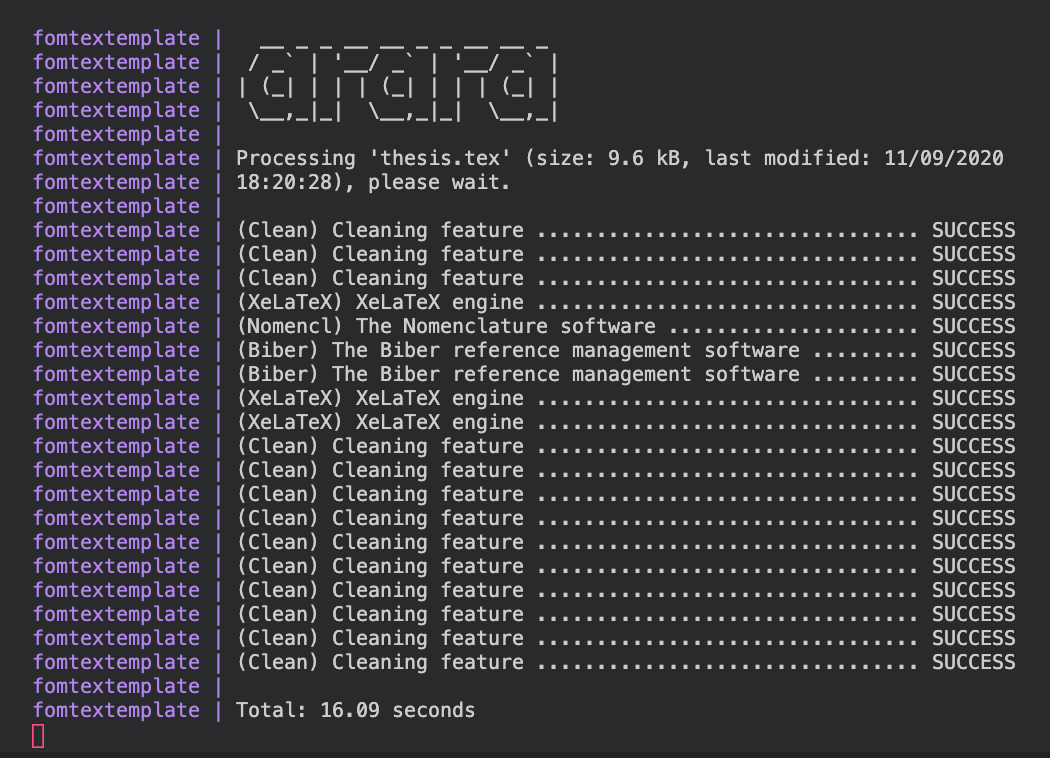
\includegraphics[width=1\textwidth]{.github/terminal}
    \captionsetup{width=1\textwidth}
    \capquelle{\cite[][200]{bsp}}\label{abb_bsp}
\end{figure}
\blindtext

\subsubsection{Design-Prinzip der Separierung von Verantwortlichkeiten}
\blindtext\footcite[Vgl. ][79]{Schelinski2019}

\begin{table}[h]
    \centering
    \begin{threeparttable}
        \centering
        \begin{tabular}{cccccccc}
            {$m$} & {$\Re\{\underline{\mathfrak{X}}(m)\}$} & {$-\Im\{\underline{\mathfrak{X}}(m)\}$} & {$\mathfrak{X}(m)$} & {$\frac{\mathfrak{X}(m)}{23}$} & {$A_m$} & {$\varphi(m)\ /\ ^{\circ}$} & {$\varphi_m\ /\ ^{\circ}$} \\
            \hline
            1  & 16.128 & +8.872 & 16.128 & 1.402 & 1.373 & -146.6 & -137.6 \\
            2  & 3.442  & -2.509 & 3.442  & 0.299 & 0.343 & 133.2  & 152.4  \\
            3  & 1.826  & -0.363 & 1.826  & 0.159 & 0.119 & 168.5  & -161.1 \\
            4  & 0.993  & -0.429 & 0.993  & 0.086 & 0.08  & 25.6   & 90     \\
            5  & 1.29   & +0.099 & 1.29   & 0.112 & 0.097 & -175.6 & -114.7 \\
            6  & 0.483  & -0.183 & 0.483  & 0.042 & 0.063 & 22.3   & 122.5  \\
            7  & 0.766  & -0.475 & 0.766  & 0.067 & 0.039 & 141.6  & -122   \\
            8  & 0.624  & +0.365 & 0.624  & 0.054 & 0.04  & -35.7  & 90     \\
            9  & 0.641  & -0.466 & 0.641  & 0.056 & 0.045 & 133.3  & -106.3 \\
            10 & 0.45   & +0.421 & 0.45   & 0.039 & 0.034 & -69.4  & 110.9  \\
            11 & 0.598  & -0.597 & 0.598  & 0.052 & 0.025 & 92.3   & -109.3 \\
            \hline
        \end{tabular}
        \begin{tablenotes}[flushleft]
        \item \normalsize{Quelle: \cite[][200]{bsp}}
        \end{tablenotes}
    \end{threeparttable}
\end{table}

\Blindtext\footcite[Vgl. ][34]{Digitaloekonomie}
\blinditemize
\blindtext\footcite[Vgl. ][511]{Tanenbaum2016}

\subsubsection{LaTeX-Befehle}
\textnormal{Normale Schrift} -
\textbf{Fett} -
\textit{Kursiv} -
\textsl{schief} -
\underline{unterstrichen} -
\textsf{Sans Serif} -
\textrm{Roman} -
\texttt{Schreibmaschine}

\section{Schluss}
\subsection{Fazit}
\Blindtext



%====================================
% Literaturverzeichnis
%====================================
\newpage
\printbibliography[nottype=online,heading=bibintoc,title={Literaturverzeichnis}]
\printbibliography[type=online,title={Internetquellen}]
%====================================
% Deine Kapitel einbinden!!!
% Deine Inhalte einbinden!!!
%====================================
\newpage
	\newpage
\pagenumbering{gobble} % Keine Seitenzahlen mehr

%-----------------------------------
% Ehrenwörtliche Erklärung
%-----------------------------------
\section*{Ehrenwörtliche Erklärung}
Hiermit versichere ich, dass die vorliegende Arbeit von mir selbstständig und ohne unerlaubte Hilfe angefertigt worden ist, insbesondere dass ich alle Stellen, die wörtlich oder annähernd wörtlich aus Veröffentlichungen entnommen sind, durch Zitate als solche gekennzeichnet habe. Ich versichere auch, dass die von mir eingereichte schriftliche Version mit der digitalen Version übereinstimmt. Weiterhin erkläre ich, dass die Arbeit in gleicher oder ähnlicher Form noch keiner Prüfungsbehörde/Prüfungsstelle vorgelegen hat. Ich erkläre mich damit nicht einverstanden, dass die Arbeit der Öffentlichkeit zugänglich gemacht wird. Ich erkläre mich damit einverstanden, dass die Digitalversion dieser Arbeit zwecks Plagiatsprüfung auf die Server externer Anbieter hochgeladen werden darf. Die Plagiatsprüfung stellt keine Zurverfügungstellung für die Öffentlichkeit dar.


\par\medskip
\par\medskip

\vspace{5cm}

\begin{table}[H]
	\centering
	\begin{tabular*}{\textwidth}{c @{\extracolsep{\fill}} ccccc}
		München, \the\day.\the\month.\the\year
		&
		% Hinterlege deine eingescannte Unterschrift im Verzeichnis /abbildungen und nenne sie unterschrift.png
		% Bilder mit transparentem Hintergrund können teils zu Problemen führen
		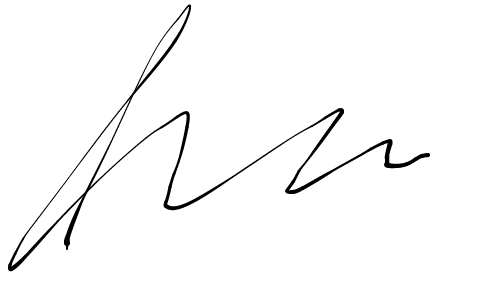
\includegraphics[width=0.35\textwidth]{unterschrift}\vspace*{-0.35cm}
		\\
		\rule[0.5ex]{12em}{0.55pt} & \rule[0.5ex]{12em}{0.55pt} \\
		(Ort, Datum) & (Eigenhändige Unterschrift)
		\\
	\end{tabular*} \\
\end{table}



%====================================

\end{document}
